\lab{The Arnoldi Iteration}{The Arnoldi Iteration}
\objective{The Arnoldi Iteration is an efficient method for finding the eigenvalues of extremely large matrices.
Instead of using standard methods, the iteration uses Krylov subspaces to approximate how a linear operator acts on vectors.
With this approach, the Arnoldi Iteration facilitates the computation of eigenvalues for enormous matrices without needing to physically create the matrix in memory.
We will explore this subject by implementing the Arnoldi iteration algorithm, using our implementation for eigenvalue computation, and then graphically representing the accuracy of our approximated eigenvalues.}

\section*{Krylov Subspaces} % =================================================

One of the biggest difficulties in numerical linear algebra is the amount of memory needed to store a large matrix and the amount of time needed to read its entries.
Methods using Krylov subspaces avoid this difficulty by studying how a matrix acts on vectors, making it unnecessary in many cases to create the matrix itself.

The \emph{Arnoldi Iteration} is an algorithm for finding an orthonormal basis of a Krylov subspace.
One of its strengths is that it can run on any linear operator without knowing the operator's underlying matrix representation.
The outputs of the Arnoldi algorithm can then be used to approximate the eigenvalues of the matrix of the linear operator.

The order-$n$ Krylov subspace of $A$ generated by $\x$ is
\[
\mathcal{K}_n(A, \x) =\text{span} \{\x, A\x, A^2\x, \ldots, A^{n-1}\x\}.
\]
If the vectors $\{\x, A\x, A^2\x, \ldots, A^{n-1}\x\}$ are linearly independent, then they form a basis for $\mathcal{K}_n(A,\x)$.
However, $A^n x$ frequently converges to a dominant eigenvector of $A$ as $n$ gets large, which fills the basis with many almost parallel vectors.
This yields a basis prone to ill-conditioned computations and numerical instability.

\section*{The Arnoldi Iteration Algorithm} % ==================================

The Arnoldi iteration focuses on efficiently creating an orthonormal basis for $\mathcal{K}_n(A,\x)$ by integrating the creation of $\{\x, A\x, A^2\x, \ldots, A^{n-1}\x\}$ with the modified Gram-Schmidt algorithm.
This process yields an orthonormal basis for $\mathcal{K}_n(A,\x)$ that can be used for further computations.
%A brief walkthrough of this method and a psuedo code representation of it are contained below.

\begin{comment}
Before discussing the specific uses of the Krylov subspace in linear systems and eigenvalue problems, let us address a very practical concern: how can we best compute a basis for the Krylov subspace?
The obvious answer is simply to calculate the vectors $x, ax, a^2x, \ldots, a^{n-1} x$, which we can accomplish using only matrix-vector multiplication.
Straightforward though this may be, there is a major problem: $a^n x$ tends to converge to a dominant eigenvector of $a$ as $n$ gets large, and consequently these vectors become nearly parallel.
Thus, the basis $\{x, ax, a^2x, \ldots, a^{n-1} x\}$ is far from orthogonal, and matrix computations associated with this basis will likely be ill-conditioned and prone to numerical instability.
To redress this problem, we may think to apply the Gram-Schmidt orthogonalization process to the basis, obtaining an orthonormal basis for the krylov subspace that enjoys much better numerical properties.
This turns out to be a useful thought, and is the basis for the Arnoldi iteration.

You may recall from lab \ref{lab:qrdecomp} that the modified Gram-Schmidt algorithm allows us to find an increasing number of orthogonal vectors but does not require that we run the algorithm to its completion to find a full basis.
Our goal is to find an orthonormal set of vectors $q_1,\ldots,q_n$ having the same span as $x, ax, a^2x, \ldots, a^{n-1} x$.
We start things off by setting
\[
q_1 = \frac{x}{\|x\|_2}.
\]
now, assuming we have obtained $q_1,\ldots,q_n$, we obtain $q_{n+1}$ by projecting $a q_n$ onto the previous vectors, subtracting out these projections, and then normalizing.
To make this more precise, let $h_{i,n} = \langle q_i, a q_n\rangle$ for $i = 1,\ldots, n$. subtract out these projections by calculating
\[
p_{n+1} = a^n x - \sum_{i=1}^n h_{i,n}q_i.
\]
define $h_{n+1,n} = \|p_{n+1}\|_2$, and normalize $p_{n+1}$ by calculating
\[
q_{n+1} = \frac{p_{n+1}}{h_{n+1,n}},
\]
our next basis vector.
This procedure is outlined (in slightly more python-friendly notation) in algorithm \ref{alg:arnoldi_iteration}.

Perhaps you noticed a slight discrepancy between the Arnoldi iteration as described above, and the usual Gram-Schmidt procedure.
Specifically, you might have expected to compute $q_{n+1}$ by projecting $a^n x$, rather than $a q_n$, onto the previous vectors.
Thankfully, it is straightforward to show that our algorithm produces a valid orthonormal basis for the Krylov subspace, despite this difference, and because of this detail, we do not need to compute and store the original Krylov basis $x, ax, \ldots, a^{n-1}x$.
Additionally, each iteration only requires one matrix-vector calculation, and the individual entries in $a$ are never referenced or modified.
Thus, even if the matrix $a$ is very large in theory, as long as we have a reasonably efficient subroutine to calculate $ax$ for any vector $x$, the Arnoldi iteration is computationally tractable.

This algorithm produces an orthonormal basis $q_1,\ldots,q_n$ for the order-$n$ Krylov subspace generated by $a$ and $x$, as well as a collection of numbers $h_{i,j}$.
If we define a matrix $h_n$ whose $i,j$'th entry is $h_{i,j}$ for $i \leq j+1$ and is $0$ otherwise, we now have an upper Hessenberg matrix.
Recall that an upper Hessenberg matrix has the property that all entries below the first subdiagonal are equal to zero.
Any square matrix is unitarily similar to an upper Hessenberg matrix.
Dealing with a Hessenberg matrix is often more convenient than dealing with a general matrix, especially when it comes to finding eigenvalues or solving systems of equations, since efficient algorithms designed for these types of matrices exist.
It turns out that there is a Hessenberg factorization of $a$, given by
\[
a  = qhq^*,
\]
Where $q$ is a unitary matrix and $h$ is upper Hessenberg such that the first $n$ columns of $q$ are $q_1,\ldots,q_n$, and the upper left $n \times n$ submatrix of $h$ is equal to $h_n$.
Hence, the Arnoldi iteration provides a connection between the Krylov subspace and the Hessenberg factorization of a matrix.
Each step in the Arnoldi iteration can be thought of as computing another step in the Hessenberg reduction of $a$.
Each $h_n$ is really just the $n \times n + 1$ upper-left block of $h$.
Solving eigenvalue problems or systems of equations for a general square matrix can thus be reduced, via Arnoldi iteration, to solving these problems for a Hessenberg matrix, a much easier task.

At this point, we can view the Arnoldi iteration as a means to compute an orthonormal basis for a Krylov subspace, or alternatively, to compute a partial Hessenberg factorization of a matrix.
But in lab \ref{lab:canonical_transformations}, we discussed how orthogonal transformations can be used to transform a matrix to upper Hessenberg form.
We were able to find the eigenvalues of such upper Hessenberg matrices in lab \ref{lab:eigsolve}.
So what have we really gained by this new approach?
These previous approaches were based on matrix-matrix multiplication and required us to manipulate individual entries of the matrix.
The Arnoldi iteration avoids this and relies only on our ability to calculate matrix-vector multiplication.
Further, our present approach will allow us to compute only a partial Hessenberg factorization.
This is advantageous when, as is often the case, the behavior and properties of a matrix can be well-approximated by only a small portion of its Hessenberg form.
\end{comment}

The algorithm begins by initializing a matrix $H$ which will be an upper Hessenberg matrix and a matrix $Q$ which will be filled with the basis vectors of our Krylov subspace.
It also requires an initial vector $\b \neq 0$ which is normalized to get $\q_1 = \b/\norm{\b}$.
This represents the basis for the initial Krylov subspace, $\mathcal{K}_1(A,\b)$.

For the $k$th iteration, compute the next basis vector $\q_{k+1}$ by using the modified Gram-Schmidt process to make $A\q_k$ orthonormal to $\q_k$.
This entails making each column of $Q$ orthogonal to $\q_k$ before proceeding to the next iteration.
The vectors $\{\q_i\}_{i=1}^k$ are then a basis for $\mathcal{K}_k(A,\b)$.
If $\norm{\q_{k+1}}$ is below a certain tolerance, stop and return $H$ and $Q$.
Otherwise, normalize the new basis vector new $\q_{k+1}$ and continue to the next iteration.
% This process continues until we have an orthonormal basis of an order $k+1$ Krylov subspace.

%This algorithm is described in algorithm \ref{alg:arnoldi_iteration} for an order $k+1$ Krylov subspace, where $k$ is the number of times we multiply by $A$.

\begin{algorithm}
\begin{algorithmic}[1]
\Procedure{Arnoldi}{$\b$, $A$, $k$, \li{tol}}
	\State $Q \gets \allocate{\size{\b}}{k+1}$			\Comment{Some initialization steps}
	\State $H \gets \zeros{ k+1}{ k}$
	\State $Q_{:,0} \gets \b/\norm{\b}_2$
	\For{$j=0\ldots k-1$}							\Comment{Perform the actual iteration.}
		\State $Q_{:,j+1} \gets A(Q_{:,j})$
		\For{$i=0\ldots j$}					\Comment{Modified Gram-Schmidt.}
			\State $H_{i,j} \gets Q_{:,i}\hrm Q_{:,j+1}$
			\State $Q_{:,j+1} \gets Q_{:,j+1} - H_{i,j} Q_{:,i}$
		\EndFor
		\State $H_{j+1,j} \gets \norm{Q_{:,j+1}}_2$			\Comment{Set subdiagonal element of $H$.}
            \If{$|H_{j+1,j}|<$ \li{tol}}					\Comment{Stop if $\norm{Q_{:,j+1}}_2$ is small enough.}
			\State \pseudoli{return} $H_{:j+1,:j+1}$, $Q_{:,:j+1}$
		\EndIf
		\State $Q_{:,j+1} \gets Q_{:,j+1}/H_{j+1,j}$				\Comment{Normalize $\q_{j+1}$.}
	\EndFor
	\State \pseudoli{return} $H_{:-1, :}$, $Q$			\Comment{Return $H_k$ and $Q$.}
\EndProcedure
\end{algorithmic}
\caption{The Arnoldi iteration.
This algorithm accepts a square matrix $A$ and a starting vector $\b$.
It iterates $k$ times or until the norm of the next vector in the iteration is less than \li{tol}.
The algorithm returns an upper Hessenberg $H$ and an orthonormal $Q$ such that $H = Q^{\mathsf{H}}AQ$.}
\label{alg:arnoldi_iteration}
\end{algorithm}

\begin{warn}
If the starting vector $\x$ is an eigenvector of $A$ with corresponding eigenvalue $\lambda$, then by definition $\mathcal{K}_k(A, \x)=\text{span}\{\x, \lambda \x, \lambda^2\x, \ldots, \lambda^k \x\}$, which is equal to the span of $\x$.
So, when $\x$ is normalized with $\q_1 = \x/\|\x\|$, $\q_2 = A\q_1 = \lambda \q_1$.

The vector $\q_2$ is supposed to be the next vector in the orthonormal basis for $\mathcal{K}_k(A, \x)$, but it is not linearly independent of $\q_1$.
In fact, $\q_1$ already spans $\mathcal{K}_k(A, \x)$.
Hence, the Gram-Schmidt process fails and results in a \li{ZeroDivisionError} or an extremely early termination of the algorithm.
A similar phenomenon may occur if the starting vector $\x$ is contained in a proper invariant subspace of $A$.
\end{warn}

\section*{Arnoldi Iteration on Linear Operators} % ============================

A major strength of the Arnoldi iteration is that it can run on a linear operator, even without knowing the matrix representation of the operator.
If $L$ is some linear function, then we can modify the pseudocode above by replacing $AQ_{:,j}$ with $A_{mul}(Q_{:,j})$.
This makes it possible to find the eigenvalues of an arbitrary linear transformation.

\begin{problem}\label{prob:arnoldi}
Write a function that accepts a starting vector $\b$ for the Arnoldi Iteration, a function handle $L$ that describes a linear operator, the number of times $n$ to perform the iteration, and a tolerance \li{tol} that defaults to $10^{-8}$.
Use Algorithm \ref{alg:arnoldi_iteration} to implement the Arnoldi Iteration with these parameters.
Return the upper Hessenberg matrix $H$ and the orthonormal matrix $Q$ from the iteration.

Consider the following implementation details.
\begin{enumerate}
\item Since $H$ and $Q$ will eventually hold complex numbers, initialize them as complex arrays (e.g., \li{A = np.empty((3,3), dtype=np.complex128)}).
\item This function can be tested on a matrix A by passing in \li{A.dot} for a linear operator.
\item Remember to use complex inner products. Here is an example of how to evaluate $A^HA$:
\begin{lstlisting}
b = A.conj() @ B
\end{lstlisting}
\end{enumerate}
Test your function by comparing the resulting $H$ with $Q\hrm A Q$.
\end{problem}

\section*{Finding Eigenvalues Using the Arnoldi Iteration} % ==================

Let $A$ be an $n \times n$ matrix.
Let $Q_k$ be the matrix whose columns $\q_1, \ldots, \q_k$ are the orthonormal basis for $\mathcal{K}_m(A, \x)$ generated by the Arnoldi algorithm, and let $H_k$ be the $k\times k$ upper Hessenburg matrix defined at the $k$th stage of the algorithm.
Then these matrices satisfy
\begin{equation}\label{eq:arnoldi-hqa}
H_k = Q_k^{\mathsf H} A Q_k.
\end{equation}
If $k<n$, then $H_k$ is a low-rank approximation to $A$  and the eigenvalues of $H_k$ may be used as approximations for the eigenvalues of $A$.
The eigenvalues of $H_k$ are called \emph{Ritz Values}, and we will later show that they converge quickly to the largest eigenvalues of $A$.

\begin{problem}\label{prob:ritz}
Write a function that accepts a function handle $L$ that describes a linear operator, the dimension of the space \li{dim} that the linear operator works on, the number of times $k$ to perform the Arnoldi Iteration, and the number of Ritz values $n$ to return.
Use the previous implementation of the Arnoldi Iteration and an eigenvalue function such as \li{scipy.linalg.eigs()} to compute the largest Ritz values of the given operator.
Return the \li{n} largest Ritz values.
\end{problem}

One application of the Arnoldi iteration is to find the eigenvalues of linear operators that are too large to store in memory.
For example, if an operator acts on a vector $\x \in \mathbb{C}^{2^{20}}$, then its matrix representation contains $2^{40}$ complex values.
Storing such a matrix would require 64 terabytes of memory!

An example of such an operator is the Fast Fourier Transform, cited by SIAM as one of the top algorithms of the century \cite{cipra2000}.
The Fast Fourier Transform is used very commonly in signal processing.

\begin{problem}
\label{prob:fourier_eigs}
The four largest eigenvalues of the Fast Fourier Transform are known to be $\{ -\sqrt{n}, \sqrt{n}, -i\sqrt{n}, i\sqrt{n} \}$ where $n$ is the dimension of the space on which the transform acts.

Use your function from Problem \ref{prob:ritz} to approximate the eigenvalues of the Fast Fourier Transform.
Set $k = 10$ and \li{dim} = $2^{20}$.
For the argument $L$, use the \li{scipy.fftpack.fft()}.
\end{problem}

The Arnoldi iteration for finding eigenvalues is implemented in a Fortran library called ARPACK.
Scipy interfaces with the Arnoldi iteration in this library via the function \li{scipy.sparse.linalg.eigs()}.
This function has many more options than the implementation we wrote in Problem \ref{prob:ritz}.
In this example, the keyword argument \li{k=5} specifies that we want five Ritz values.
Note that even though this function comes from the \li{sparse} library in Scipy, we can still call it on regular Numpy arrays.

\begin{lstlisting}
>>> from scipy.sparse import linalg as spla
>>> B = np.random.random((100,100))
>>> spla.eigs(B, k=5, return_eigenvectors=false)
array([ -1.15577072-2.59438308j,  -2.63675878-1.09571889j,
        -2.63675878+1.09571889j,  -3.00915592+0.j        ,  50.14472893+0.j ])
\end{lstlisting}

\subsection*{Convergence} % ---------------------------------------------------
As more iterations of the Arnoldi method are performed, our approximations are of higher rank.
Consequently, the Ritz values become more accurate approximations to the eigenvalues of the linear operator.

This technique converges quickly to eigenvalues whose magnitude is distinctly larger than the rest.
For example, matrices with random entries tend to have one eigenvalue of distinctly greatest magnitude.
Convergence of the Ritz values for such a matrix is plotted in Figure \ref{fig:arnoldi_random_val_conv}.

However, Ritz values converge more slowly for matrices with random eigenvalues.
Figure \ref{fig:arnoldi_random_eig_conv} plots convergence of the Ritz values for a matrix with eigenvalues uniformly distributed in $[0,1)$.

\begin{figure}
\centering
\begin{subfigure}[b]{.49\textwidth}
    \centering
    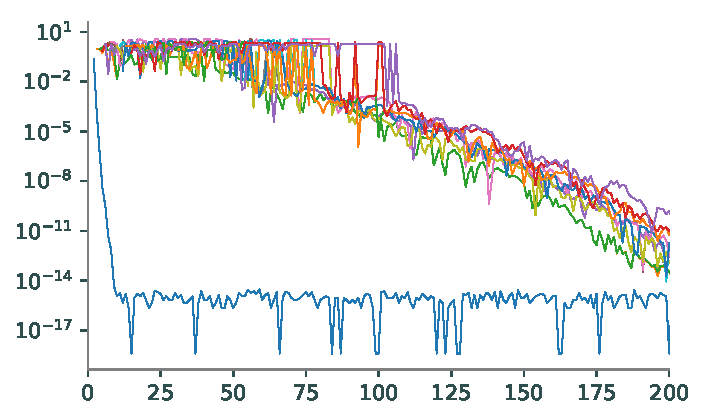
\includegraphics[width=\textwidth]{figures/rand_vals_conv.pdf}
    \caption{}
    \label{fig:arnoldi_random_val_conv}
\end{subfigure}
\begin{subfigure}[b]{.49\textwidth}
    \centering
    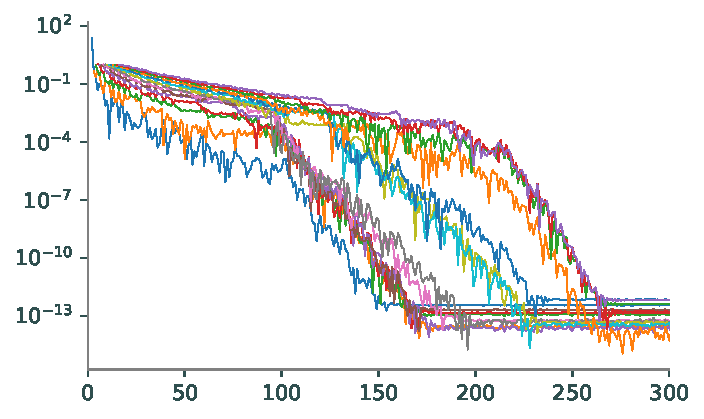
\includegraphics[width=\textwidth]{figures/rand_eigs_conv.pdf}
    \caption{}
    \label{fig:arnoldi_random_eig_conv}
\end{subfigure}
\caption{These plots show the relative error of the ritz values as approximations to the eigenvalues of a matrix.
The figure on the left plots the largest 15 Ritz values for a $500\times 500$ matrix with random entries and demonstrates that the largest eigenvalue (the blue line) converges after 20 iterations.
The figure at right plots the largest 15 Ritz values for a $500\times 500$ matrix with uniformly distributed eigenvalues in $[0,1)$ and demonstrates that all the eigenvalues take from 150 to 250 iterations to converge.}
\end{figure}

% todo: this problem may be too difficult but we have added a great deal of supplementary code to make it more doable.
\begin{problem}
Write a function that accepts a linear operator $A$, the number of Ritz values to plot $n$, and the the number of times to perform the Arnoldi iteration \li{iters}.
Use these parameters to create a plot of the absolute error between the largest Ritz values of $A$ and the largest eigenvalues of $A$.
\begin{enumerate}
    \item Find $n$ eigenvalues of $A$ of largest magnitude. Store these in order.
    \item Create an empty array to store the relative errors for every $k=0,1,\ldots,$ \li{iters}.
    \begin{enumerate}
    	\item Use your Ritz function to find the $n$ largest Ritz values of the operator. Note that for small $k$, the matrix $H_k$ may not have this many eigenvalues. Due to this, the graphs of some eigenvalues have to begin after a few iterations.
        \item Store the absolute error between the eigenvalues of A and the Ritz values of H. Make sure that the errors are stored in the correct order.
    \end{enumerate}
    %\item Use array broadcasting to compute the absolute error.
    \item Iteratively plot the errors for each eigenvalue with the range of the iterations.
\end{enumerate}
Hints:
If $\tilde{\x}$ is an an approximation to $\x$, then the \emph{absolute error} in the approximation is $\|\x - \tilde{\x}\|$.

Sort your eigenvalues from greatest to least.
An example of how to do this is included:
\begin{lstlisting}
# Evaluate the eigenvalues
eigvalues = la.eig(A)[0]
# Sort them from greatest to least (use np.abs to account for complex parts)
eigvalues = eigvalues[np.sort(np.<<abs>>(eigvalues))[::-1]]
\end{lstlisting}
In addition, remember that certain eigenvalues of $H$ will not appear until we are computing enough iterations in the Arnoldi algorithm.
As a result, we will have to begin the graphs of several eigenvalues after we are computing sufficient iterations of the algorithm.
%To be able to keep our graph readable, use masking such as the following to remove any extreme errors that arise in the first iterations.
%\begin{lstlisting}
%errors[errors > 10] = 10.
%\end{lstlisting}

Run your function on these examples.
The plots should be fairly similar to Figures \ref{fig:arnoldi_random_eig_conv} and \ref{fig:arnoldi_random_val_conv}.

\begin{lstlisting}
>>> A = np.random.rand(300, 300)
>>> plot_ritz(a, 10, 175)

>>> # A matrix with uniformly distributed eigenvalues
>>> d = np.diag(np.random.rand(300))
>>> B = A @ d @ la.inv(A)
>>> plot_ritz(B, 10, 175)
\end{lstlisting}
% These may take some time to run.
\end{problem}

% once the eigenvalue lab has been rewritten, have them use their own solver to find the eigenvalues of the $h_k$.

% this problem is very ill-conditioned.
\begin{comment}
\begin{problem}
finding the roots of a polynomial can be represented as an eigenvalue problem.
finding the roots of a monic polynomial (a polynomial with leading coefficient 1) $p = c_0 + c_1 x + \dots + c_{n-1} x^{n-1} + x^n$ is equivalent to finding the eigenvalues of the matrix
\[c = \begin{bmatrix}
0 & 0 & \dots & 0 & -c_0 \\
1 & 0 & \dots & 0 & -c_1 \\
0 & 1 & \dots & 0 & -c_2 \\
\vdots & \vdots & \ddots & \vdots & \vdots \\
0 & 0 & \dots & 1 & -c_{n-1} \end{bmatrix}\]
this matrix is called the companion matrix of the polynomial $p$.
as it happens, every matrix is similar to the companion matrix of its characteristic polynomial, but we won't use that fact here.

The following is a function that, given an array containing the coefficients $c_0, c_1, \dots, c_{n-1}$ for a monic polynomial $p$, performs matrix multiplication by the corresponding companion matrix.

\begin{lstlisting}
def companion_multiply(c, u):
    v = np.empty_like(u)
    v[0] = - c[0] * u[-1]
    v[1:] = u[:-1] - c[1:] * u[-1]
    return v
\end{lstlisting}

Use the Arnoldi iteration to estimate the five zeros of largest norm of a degree $1000$ monic polynomial with randomly chosen coefficients (the leading coefficient still needs to be 1).
Run $50$ steps of the Arnoldi iteration.
Compare your results with the roots of the polynomial computed using NumPy's \li{poly1d} class.
This computation can be done like this (where \li{c} is the array of random coefficients for the polynomial)

\begin{lstlisting}
p = np.poly1d([1] + list(c[::-1]))
roots = p.roots
# Now sort by absolute value from largest to smallest
roots = roots[np.<<abs>>(roots).argsort()][::-1]
\end{lstlisting}

How close are the first few zeros of largest norm?
\end{problem}
\end{comment}

\newpage

\section*{Additional Material} % ==============================================

\subsection*{The Lanczos Iteration} % -----------------------------------------

The Lanczos iteration is a version of the Arnoldi iteration that is optimized to operate on symmetric matrices.
If A is symmetric, then \eqref{eq:arnoldi-hqa} shows that $H_k$ is symmetric and hence tridiagonal.
This leads to two simplifications of the Arnoldi algorithm.

First, we have $0=H_{k, n}=\langle \q_k, A\q_n \rangle$ for $k \leq n-2$; i.e., $A\q_n$ is orthogonal to $\q_1, \ldots, \q_{n-2}$.
Thus, if the goal is only to compute $H_k$ (say to find the Ritz values), then we only need to store the two most recently computed columns of $Q$.
Second, the data of $H_k$ can also be stored in two vectors, one containing the main diagonal and one containing the first subdiagonal of $H_k$
(by symmetry, the first superdiagonal equals the first subdiagonal of $H_k$).

\begin{algorithm}[H]
\begin{algorithmic}[1]
\Procedure{Lanczos}{$\b, A, k, tol$}
	\State $\q_0 \gets \zeros{\size{\b}}$								\Comment{Some initialization}
	\State $\q_1 \gets \b/\norm{\b}_2$
	\State $\x \gets \allocate{k}$
	\State $\y \gets \allocate{k}$
	\For{$i=0\ldots k-1$}									\Comment{Perform the iteration.}
		\State $\z \gets A\q_1$					\Comment{$\z$ is a temporary vector to store $\q_{i+1}$.}
		\State $\x[i] \gets \q_1\trp \z$				\Comment{$\q_1$ is used to store the previous $\q_i$.}
		\State $\z \gets \z - \x[i] \q_1 + \y[i-1] \q_0$				\Comment{$\q_0$ is used to store $\q_{i-1}$.}
		\State $\y[i] = \norm{\z}_2$						\Comment{Initialize $\y[i]$.}
		\If{$\y[i]<tol$}								\Comment{Stop if $\norm{ \q_{i+1}}_2$ is too small.}
			\State \pseudoli{return} $\x[: i+1]$, $\y[: i]$
		\EndIf
		\State $\z = \z/ \y[i]$
		\State $\q_0, \q_1 = \q_1, \z$						\Comment{Store new $\q_{i+1}$ and $\q_i$ on top of $\q_1$ and $\q_0$.}
	\EndFor
	\State \pseudoli{return} $\x$, $\y[: -1]$
\EndProcedure
\end{algorithmic}
\caption{The Lanczos Iteration. This algorithm operates on a vector $\b$ of length $n$ and an $n \times n$ symmetric matrix $A$. It iterates $k$ times or until the norm of the next vector in the iteration is less than $tol$. It returns two vectors $\x$ and $\y$ that respectively contain the main diagonal and first subdiagonal of the current Hessenberg approximation.}
\label{alg:lanczos_iteration}
\end{algorithm}

\begin{comment}
\begin{problem}
\label{prob:lanczos}
Implement Algorithm \ref{alg:lanczos_iteration} by completing the following function.
Write it so that it can operate on complex arrays.
\begin{lstlisting}
def lanczos(b, L, k, tol=1E-8):
    '''Perform `k' steps of the Lanczos iteration on the symmetric linear
    operator defined by `L', starting with the vector 'b'.

    INPUTS:
    b    - A NumPy array. The starting vector for the Lanczos iteration.
    L - A function handle. Should describe a symmetric linear operator.
    k    - Number of times to perform the Lanczos iteration.
    tol  - Stop iterating if the next vector in the Lanczos iteration has
          norm less than `tol'. Defaults to 1E-8.

    RETURN:
    Return (alpha, beta) where alpha and beta are the main diagonal and
    first subdiagonal of the tridiagonal matrix computed by the Lanczos
    iteration.
    '''
\end{lstlisting}
\end{problem}
\end{comment}

As it is described in Algorithm \ref{alg:lanczos_iteration}, the Lanczos iteration is not stable.
Roundoff error may cause the $\q_i$ to be far from orthogonal.
In fact, it is possible for the $\q_i$ to be so adulterated by roundoff error that they are no longer linearly independent.
% If needed we could make a separate lab on the Lanczos iteration and the Implicitly Restarted Lanczos Method.
% There isn't time or space here for it though.

\begin{comment}
\begin{problem}
The following code performs multiplication by a tridiagonal symmetric matrix.

\begin{lstlisting}
def tri_mul(a, b, u):
   ''' Return Au where A is the tridiagonal symmetric matrix with main
   diagonal a and subdiagonal b.
   '''
    v = a * u
    v[:-1] += b * u[1:]
    v[1:] += b * u[:-1]
    return v
\end{lstlisting}

Let $A$ be a $1000\times 1000$ symmetric tridiagonal matrix with random values in its nonzero diagonals.
Use the function \li{lanczos()} from Problem \ref{prob:lanczos} with 100 iterations to estimate the 5 eigenvalues of $A$ of largest norm.
Compare these to the 5 largest true eigenvalues of $A$

If you do this problem for different vectors $a$ and $b$, you may notice that occasionally the largest Ritz value is repeated.
This happens because the vectors used in the Lanczos iteration may not be orthogonal.
These erroneous eigenvalues are called ``ghost eigenvalues.''
%They generally converge to actual eigenvalues of the matrix and can make the multiplicity of an eigenvalue look higher than it really is.
\end{problem}
\end{comment}

There are modified versions of the Lanczos iteration that are numerically stable.
One of these, the Implicitly Restarted Lanczos Method, is found in SciPy as \li{scipy.sparse.linalg.eigsh()}.
